\section{A Multi-Channel Sparse Blind Deconvolution approach to STM}

In this chapter, we will introduce our approach to address the \ac{MC-SBD} problem. We will first analyze the bi-linear nature of \ac{MC-SBD}, and overview the possible methods that address it. We then briefly introduce the Riemannian Trust Region method (RTRM), a direct non-convex optimization algorithm that addresses the \ac{SBD} problem. Finally, we present our algorithm which extends \ac{RTRM} to multiple-channel cases. 

\ac{MC-SBD}, also known as the joint sparse blind deconvolution/demixing problem is a bi-linear problem, that is, the observed signal is modeled as a convolution (or equivalent linear operation) between pairs of two unknowns—and this operation is linear in each variable when the other is fixed, but not jointly linear. Bi-linear problems can be solved by either a lifted method or a direct method. A lifted method can formulate the initial bi-linear mapping of two unknowns to a linear mapping of a single unknown, by defining a one-to-one mapping from two unknowns to the targeted unknown. For example, given observation $y = \mathbb{A}(x,h)$, where $x \in \mathbb{R}^n$ and $h \in \mathbb{R}^m$ are two inputs we try to recover. We can define an outer product $X = xh^T\in \mathbb{R}^{n\times m}$, and rewrite observation $y = \mathbb{A'}(X)$. In the case of convolution, $\mathbb{A'}$ is the Lifted circular convolution operator. A lifted problem can be solved analytically, and since we are dealing with only one subspace defined by $X$, by assigning constraints on $(x,h)$,  $X$ usually present some internal structures, and we are left with a fully convex problem; thus, the convergence to global minimum can usually be proven, this is also known as the recovery guarantee. For example, Flinth et al. show that, given both inputs are sparse, they can achieve high probability recovery by lifting the \ac{MC-SBD} problem and applying a hierarchical sparsity framework[tocite]. 

However, in real cases, it is rare to find both inputs sparse. Moreover, the lifting method is normally computationally inefficient, as the dimension of output space is the product of two separate inputs, it expands quickly with higher input dimensions, making it unfavorable for larger size problems like the QPI-STM recovery, note that it is even more expensive in the multi-channel case, as now the dimension of output space is not only product of two input space but product of $2 \cdot types$ input spaces. On the contrary, a direct method updates one input while assuming the other one is fixed, the optimization space of the problem thus grows linearly with the input dimension. The trade-off is that with direct methods, recovery guarantee is hard to obtain, instead, local minimal recovery can be guaranteed with careful algorithm design. Local convergence can be combined with an initial guess that is close to the global minimum; this recipe of combining a good initial guess and an algorithm with strong guarantees of local convergence usually leads to good recovery. 

Our algorithm is a direct method that follows the above recipe, it utilizes Riemannian Trust Region Method(RTRM) to provide local convergence. Standard Trust Region Method is a second-order method that guarantees local minimum recovery, as long as the objective(ie, the cost function $\phi$) has no degenerate stationary points, that is, the Hessian $\Delta^2\phi$ has no zero eigenvalues. This ensures a sufficiently curved optimization landscape for the algorithm to make consistent progress. Moreover, compared to first-order methods based on gradient descent, Trust Region Methods has significantly faster convergences and a better overall tail convergence when the iterates are close to local minima. 

\ac{RTRM} is first raised by Absil et al. in 2007 as the extension of Trust Region Methods on a Riemannian sub-manifold, embedded in Euclidean spaces. This is advantageous since enforcing our manifold to follow certain geometry, for example in our case, we enforce the kernel to live on a hypersphere $S$ defined by Equation \ref{hypersphere}, which removes the scaling symmetry we discussed. As a result, the \ac{RTRM} provides strong guarantees that a local minimum of the objective be attained over S. We now present the \ac{RTRM} algorithm used by Cheung et al. \cite{cheungDictionaryLearningFouriertransform2020} that addresses \ac{SBD} problem; we then build on it and present our \ac{MC-SBD} algorithm. 

\subsection{SBD algorithm}
Recall we have the objective function $\phi_{\lambda}$: 
\begin{equation}
	\phi_{\lambda} = \frac{1}{2}\left\lVert A_0 * X_0 - Y \right\rVert^2_F + \lambda \cdot  \left\lVert X\right\rVert_1,
\end{equation}
since \ac{RTRM} is a second-order method, we need to make make our objective function smooth, more particular, we need to smooth the sparse regularizer. This can be achieved by approximate the $l_1-norm$ by $r_{\mu}(X)$:
\begin{equation}
	r_{\mu}(X) \equiv \sum_{i,j} \mu^2(\sqrt{1+\mu^{-2}\cdot X_{i,j}}-1), 
\end{equation}
this is called a pseudo-Huber regularizer, in the limit of $\mu -> 0$, the regularizar resembles $l_1-norm$, in our case, we choose $\mu = 10^{-6}$. 

To adopt a direct method as we discussed, we will updates each input to minimize the objective function while assuming the other input fixed. We now solve: 
\begin{equation}
	\label{sbdalgorithm}
	(\hat{A}, \hat{X}) \leftarrow \min_{{A} \in {S}} \left\{ 
	\phi_{\lambda}({A}) \equiv \min_{X} \left[ 
	\phi_{\lambda}({A}, {X}) \equiv \frac{1}{2} \left\| {A} * {X} - {Y} \right\|_F^2 
	+ \lambda \cdot r_{\mu}({X}) 
	\right] 
	\right\}.
\end{equation}
This updating algorithm consists of an inner and an outer solver. The inner solver: $X \leftarrow \mathbf{XSolve}(A, \lambda)$, that is, obtaining $\hat{X}$ that minimizes $\phi_{\lambda}(A,X)$ using \ac{RTRM}. The outer solver: $A \leftarrow \mathbf{ASolve}(A, \hat{X}, \lambda)$, updating $A$ that minimizes $\phi_{\lambda}(A,X)$ using \ac{RTRM}. Since $\mathbf{XSolve}$ is an intermediate step, for $i^{th}$ iteration, we can simply write the process as: $(A^{i+1}, X^{i+1}) \leftarrow \mathbf{ASolve}(A^{i}, X^{i}, \lambda; Y,(m_1,m_2))$, where $(m_1,m_2)$ is the predefined kernel size. Or for a complete process of in total n such loops, we write $(A, X) \leftarrow \mathbf{ASolve}^n(A, X, \lambda; Y,(m_1,m_2))$

We can then write the Complete SBD-STM procedure: 

\begin{algorithm}
	\label{SBDalgo}
	\caption{Complete SBD-STM Procedure}
	\textbf{Input:}
	\begin{itemize}
		\item Observation $Y \in \mathbb{R}^{n_1 \times n_2 \times s}$,
		\item Kernel size $(m_1, m_2)$,
		\item Initial $\lambda_0 \geq 0$, decay rate $\alpha \in [0,1)$, and final $\lambda_{\text{end}} \geq 0$.
	\end{itemize}
	
	\textbf{Phase I:}
	\begin{enumerate}
		\item Randomly initialize: $A^{(0)} \in S = \mathbb{S}^{m_1 \times m_2 \times s}$.
		\item $A_\star^{(0)} \leftarrow \texttt{ASolve}^N(A^{(0)}, \lambda_0, loop)$.
	\end{enumerate}
	
	\textbf{Phase II:}
	\begin{enumerate}
		\item Lifting: Get $A^{(1)} \in S' = \mathbb{S}^{m_1' \times m_2' \times s}$ by zero-padding the edges of $A_\star^{(0)}$ with a border of width $\left\lfloor \frac{m_1}{2} \right\rfloor$.
		\item Set $\lambda_1 = \lambda_0$.
		\item Refinement: \textbf{Repeat} for $k = 1, 2, \dots$ \textbf{until} $\lambda_k \leq \lambda_{\text{end}}$,
		\begin{enumerate}
			\item[(a)] $A_\star^{(k)} \leftarrow \texttt{ASolve}^N(A^{(k)}, \lambda_k)$,
			\item[(b)] \textbf{Centering}:
			\begin{enumerate}
				\item[i.] Find the size $m_1 \times m_2$ submatrix of $A_\star^{(k)}$ that maximizes the Frobenius (square) norm across all $m_1 \times m_2$ submatrices.
				\item[ii.] Get $A^{(k+1)}$ by shifting $A_\star^{(k)}$ so that the chosen $m_1 \times m_2$ restriction is in the center, removing and zero-padding entries as needed.
				\item[iii.] Normalize $A^{(k+1)}$ so it lies in $S'$.
			\end{enumerate}
			\item[(c)] Set $\lambda_{k+1} = \alpha \lambda_k$.
		\end{enumerate}
	\end{enumerate}
	
	\textbf{Output:}
	\begin{itemize}
		\item Extract $\hat{A} \in S$ by extracting the restriction of the final $A^{(k+1)}$ to the center $m_1 \times m_2$ window.
		\item Find the corresponding activation map $\hat{X} \in \mathbb{R}^{n_1 \times n_2}$ by solving $\min_{X} \psi_{\lambda_k}(\hat{A}, X)$.
	\end{itemize}
\end{algorithm}

The kernel $A^{(0)}$ is first randomly initialized and normalized, it is then fed into two phases sequentially. Both phases utilize the same core algorithm $\mathbf{ASolve}$ as described above. Phase I aims to obtain a primary kernel $A^{(0)}_*$ given $\lambda_0$. Phase II serves as a refinement that increases the recovery quality by applying a stricter sparsity regularizer $\lambda_{k} > \lambda_0$, as well as addresses the degeneracy brought by the translation symmetry formulated in Equation \ref{translational_symm}. The latter is achieved by applying a so-called shift-truncate method, as illustrated in Figure. \ref{fig:ch6_phase2}. This method lifts the primary kernel $A^{(0)}_*$ by zero padding its edge with zeros to get a padded kernel with bigger size $(m_1',m_2')$, the padded kernel is then fed into $\mathbf{ASolve}$ with stricter $\lambda_{k}$ and get $A^{(k)}_*$ as shown in b). The Frobenius square norms are calculated on all the possible submatrices with size $(m_1,m_2)$ within $A^{(k)}_*$. An example of the submatrix window is illustrated in red square in b), and we can generate a heat map as shown in c), with each pixel in the heat map corresponding to a submatrix. The algorithm then finds the submatrix that maximizes the norm, which corresponds to the red cross in c), and we then truncate according to this submatrix and normalize it to get $A^{(k+1)}$. 

Using the Frobenius square norm score in the shift-truncate method is common practice and works well in most cases. However, it fails in more complicated situations, especially when we have other features in the padded kernel, this is illustrated in Figure. \ref{fig:ch6_phase2mod}, given primary kernel $A^{(0)}_*$, we pad it and apply $\mathbf{ASolve}$ to get $A^{(1)}_*$. The Frobenius square norm score is shown in c) and by picking the maximum, we get e), which resembles the primary kernel. This issue is mainly due to faint features around the primary feature. We can improve this algorithm by applying a radial decay term $\eta_d(r) = e^{-lnd \cdot r}$ to the Frobenius square norm, where r is the normalized distance from the submatrix window center, and d is the tunable decay factor. This biases the center features and is consistent with the decaying nature of the QPI patterns. With this decay term (d=2) applied, we obtain a heat map $S'$ as shown in d), and a truncated kernel $A^{(1)'}$ in f) has the primary more centered compared to e). For convenience, unless otherwise mentioned, all phase II that we introduced later will be using the center-biased Frobenius square norm. 

\begin{figure}
	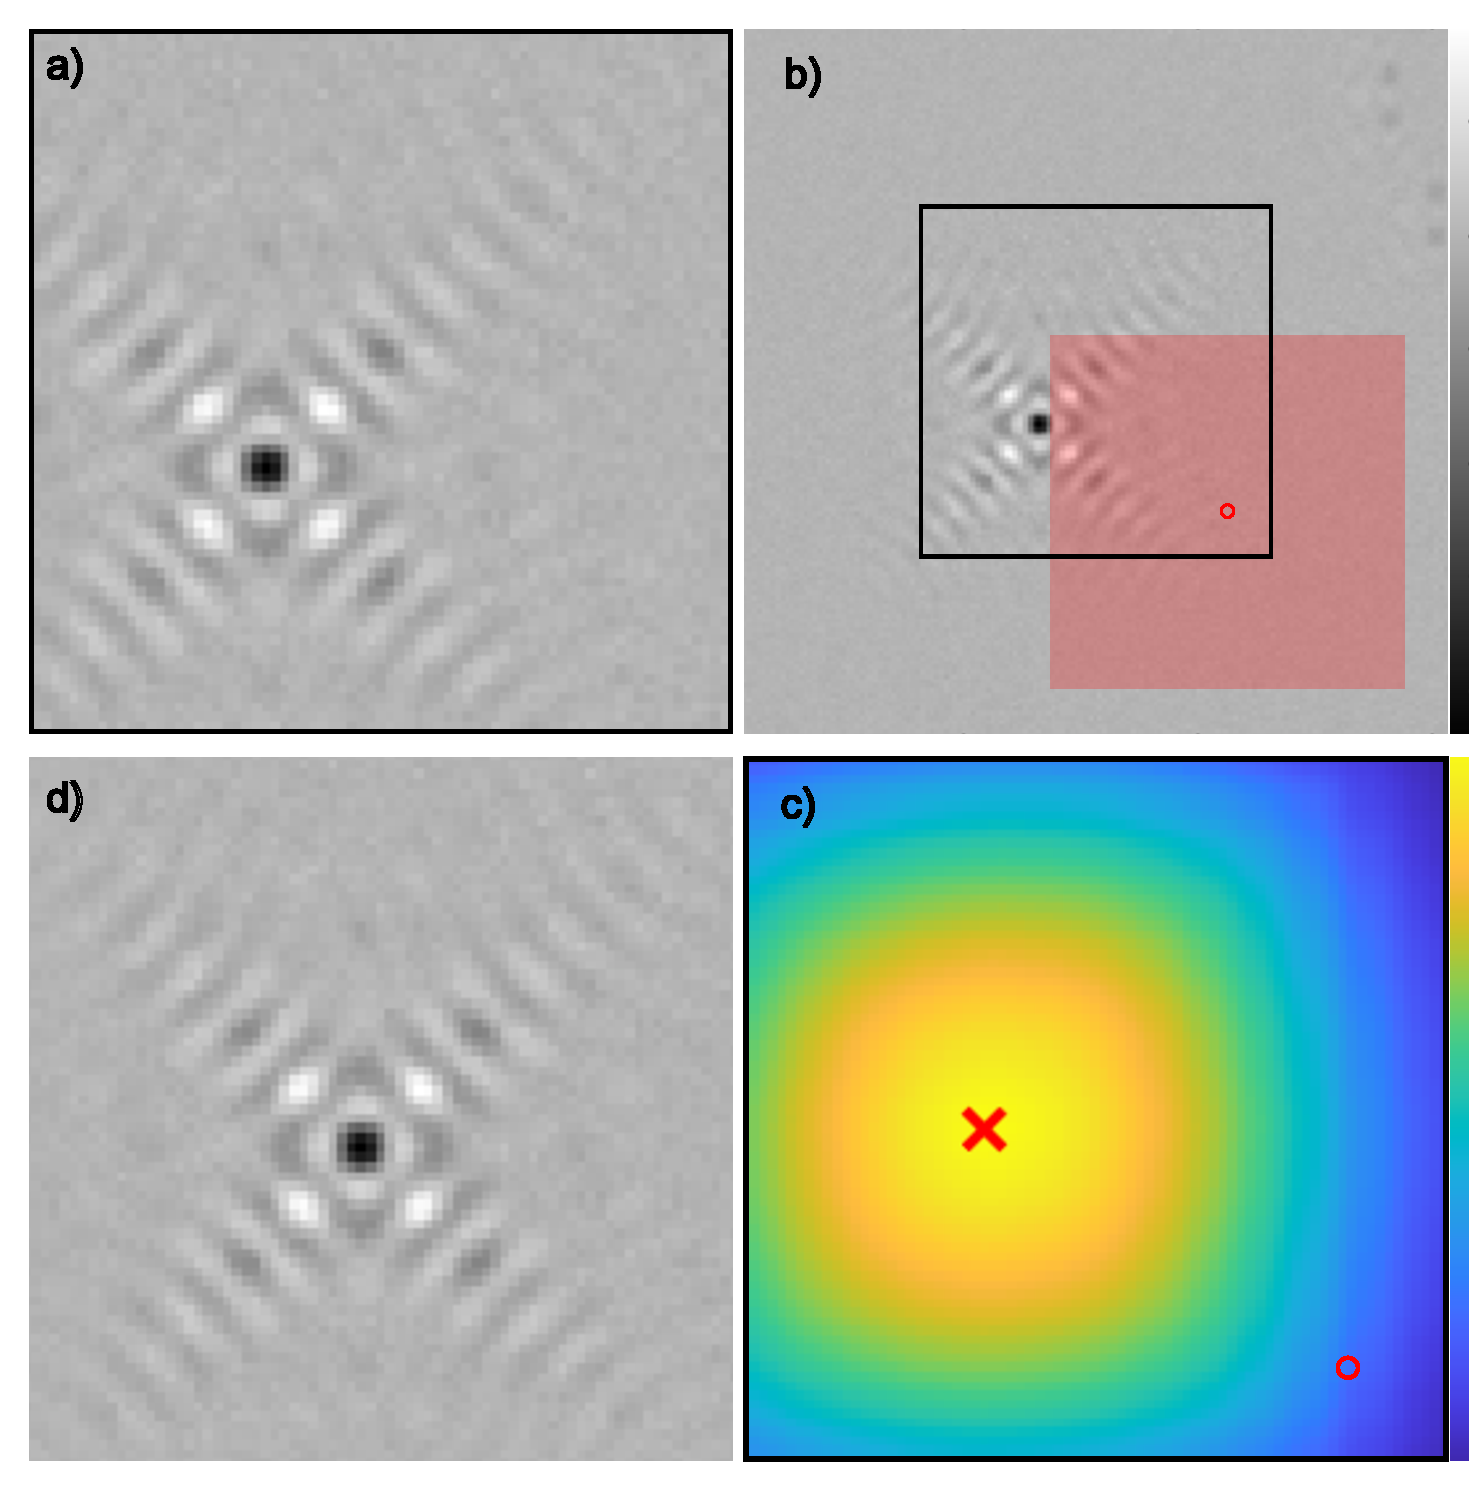
\includegraphics[width= \textwidth]{phase2old.pdf}
	\centering
	\caption{}
	\label{fig:ch6_phase2}
\end{figure}


\begin{figure}
	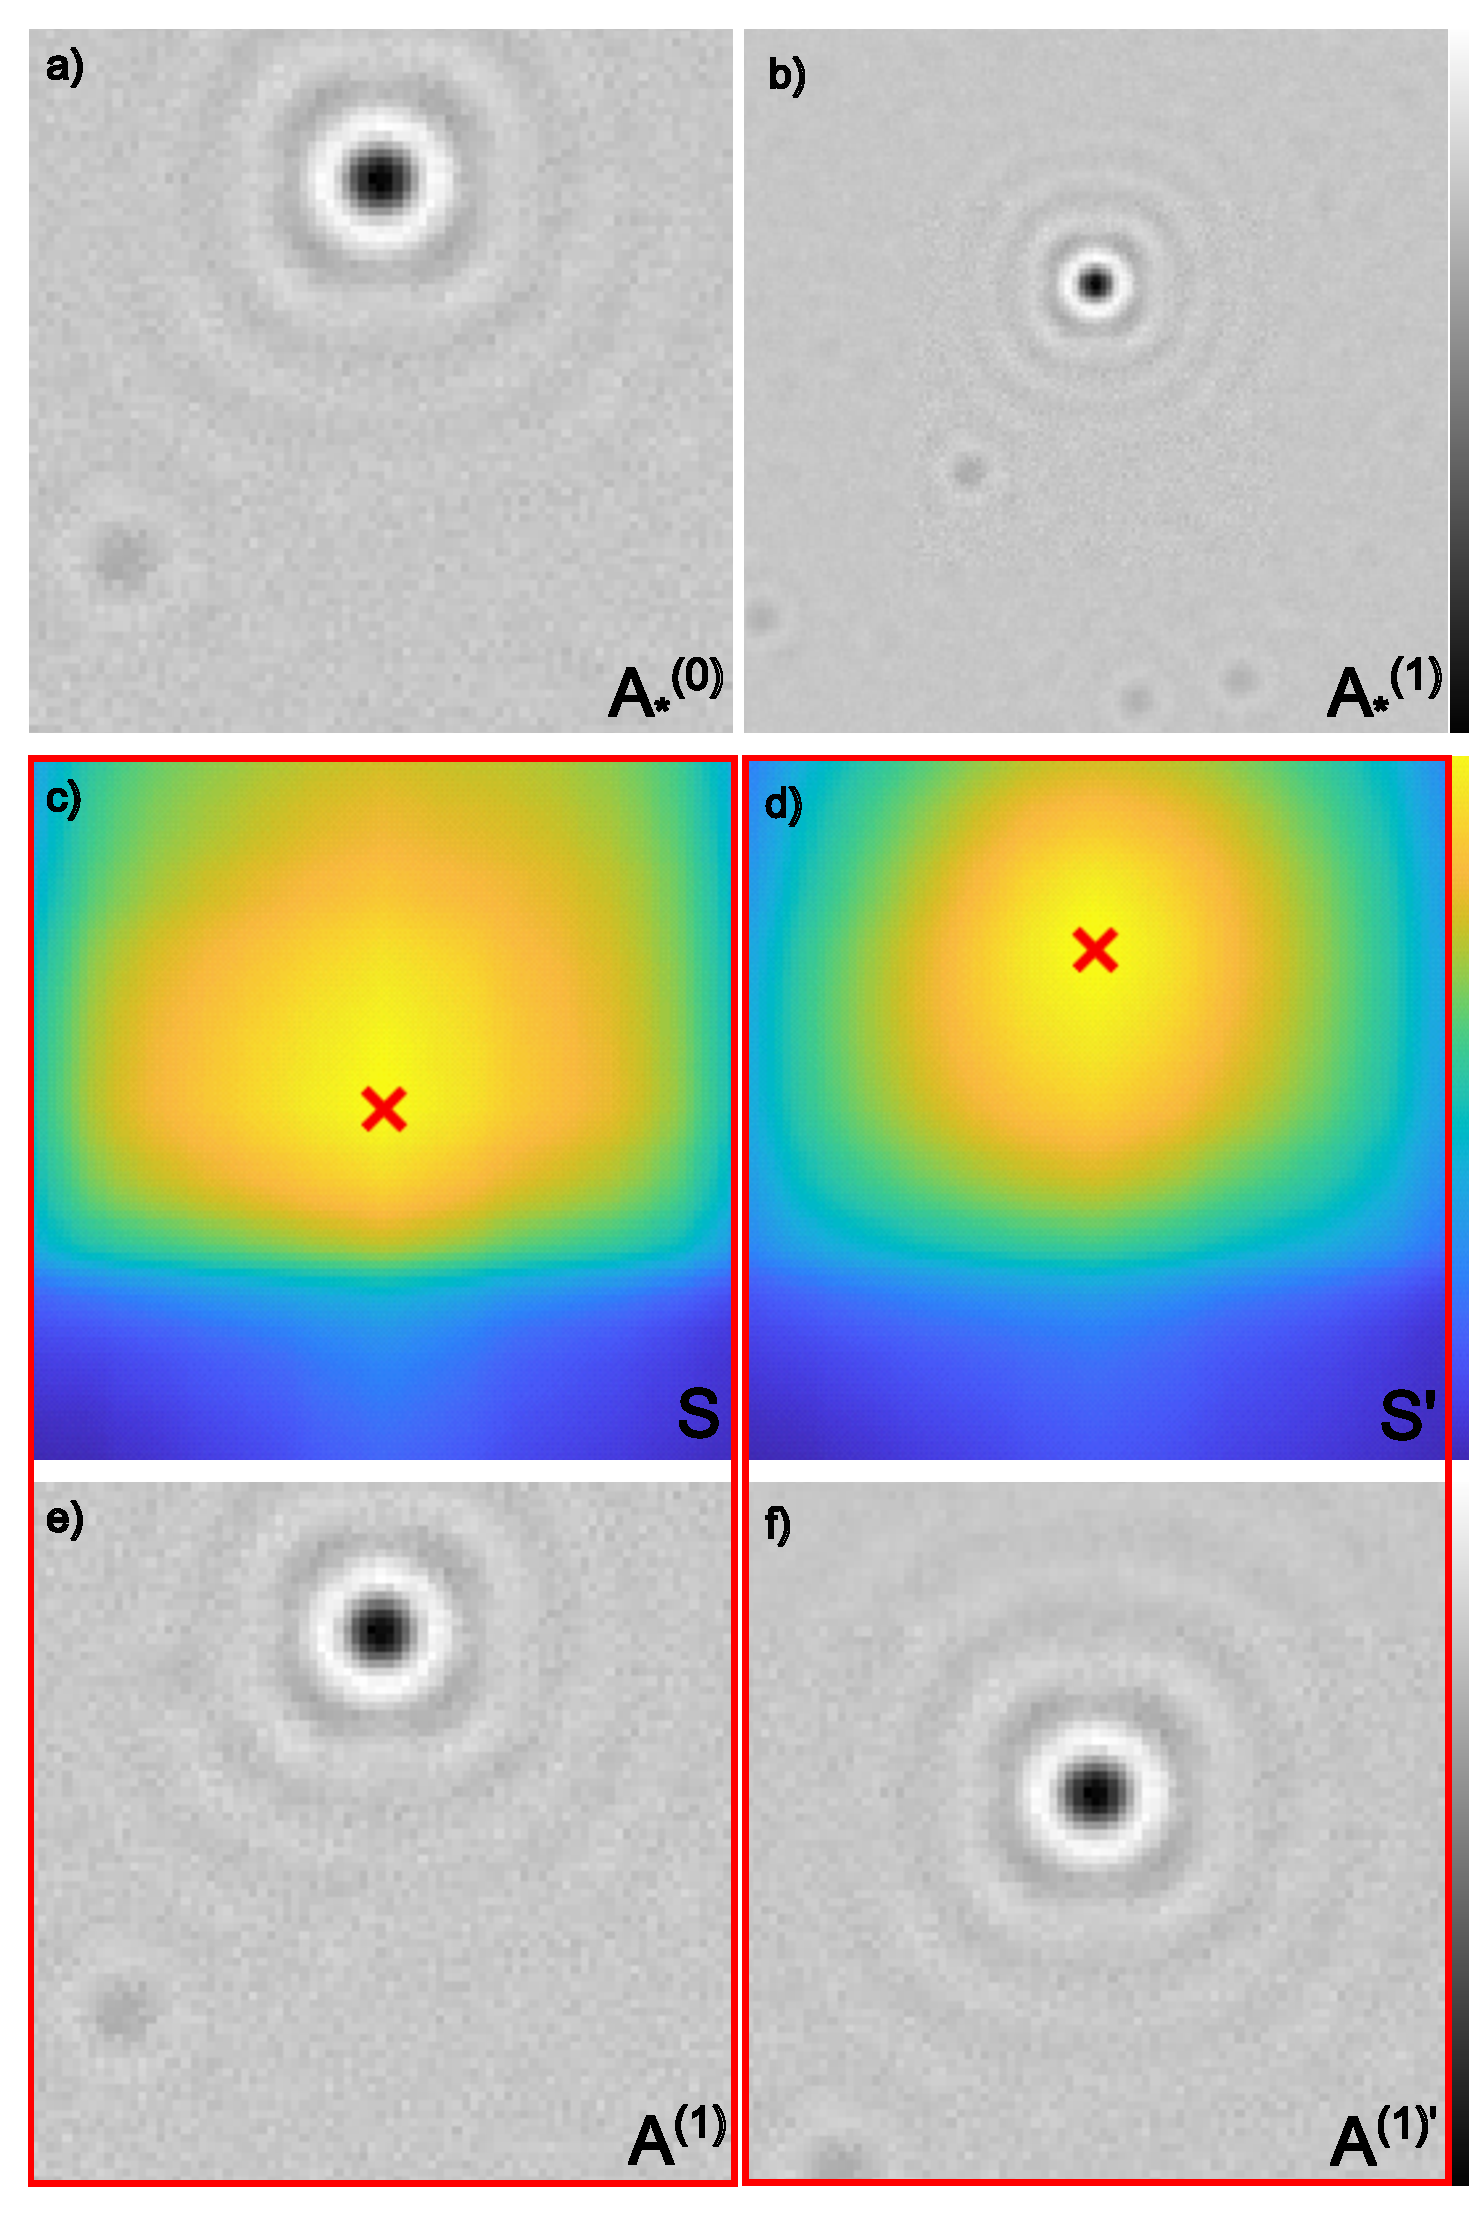
\includegraphics[width= \textwidth]{phase2mod.pdf}
	\centering
	\caption{}
	\label{fig:ch6_phase2mod}
\end{figure}


\subsection{MC-SBD algorithm}
We first establish some intuition about the multi-channel blind deconvolution process. Consider a generation process of the observation $Y$: 
\begin{equation}
	\label{eq:dec}
	Y = \sum_{i}^{s} A_i^{gt} * X_i^{gt} + noise, 
\end{equation}
\noindent where the superscript $gt$ indicate the ground truth. \ac{MC-SBD} aims to deconvolute multiple kernel-activation pairs given observation $Y$, such that $A_i=A_i^{gt}$ and $X_i = X_i^{gt}$, for all types $i \in [1,2,...,s]$. We can rewrite Equation \ref{eq:dec} as: 
\begin{align}
	Y &= \sum_{i}^{s} Y_i^{gt} + noise,\\ 
	Y_i^{gt} &= A_i^{gt} * X_i^{gt}.
\end{align}
\noindent This hints at the two separate operations in the data generation process: convolution and composition. Therefore, our \ac{MC-SBD} follows the reverse order: we first decompose the observation into kernel-specific components and then deconvolute each component into its kernel and activation. 

Due to the two-stage nature of the process, we adopt a hierarchical direct treatment across both the intra-type and the inter-type levels. At the intra-type level, when updating a specific kernel $A_j$, we hold its corresponding activation $X_j$ fixed -- a strategy inherited from the single-type \ac{SBD} algorithm. At the inter-type level, when handling the $j$-th type, we treat all $Y_i, i\neq j$ as fixed. 

This hierarchical approach enables isolated analysis for each type’s recovery:
\begin{align}
	Y_j &= Y - [\sum_{i\neq j}Y_i + noise],\\
	A_j * X_j &= Y - [\sum_{i\neq j}Y_i + noise].
\end{align} 
\noindent We can then write $Y_i = Y_i^{gt}- Y_i^{residual}$ and substitute the observation with \ref{eq:dec}. Then we have:
\begin{align}
	A_j * X_j &= \sum_{i}^{s} Y_i^{gt} + noise' - [\sum_{i\neq j}(Y_i^{gt}- Y_i^{residual}) + noise],\\ \label{eq:622}
	A_j * X_j &= Y_j^{gt}+ \sum_{i\neq j}Y_i^{residual} + noise = Y_j,
\end{align} 

\noindent The combined noise terms are absorbed into a single term. Equation \ref{eq:622} now resembles a single blind deconvolution problem, which can be addressed using the \ac{SBD} algorithm.

Smaller $Y_i^{residual}$ values for all $i \neq j$ lead to better-posed subproblems for each type. Consequently, when updating with the \ac{SBD} algorithm, we can produce a result $Y_j = A_j* X_j$ that is closer to the true component $Y_j^{gt}$. This motivates a loop structure in our algorithm: by updating one type (e.g. $j$), we reduce its residual $Y_j^{residual}$, which in turn helps improve the subsequent recovery of another type $i \neq j$. Through iterative refinement, given the local convergence guarantees provided by the \ac{RTRM} method, the residuals across all types could be gradually minimized, allowing the full reconstruction to converge towards the ground truth. However, this logic can break down in the early stages of optimization, where the residuals are large and noisy—making it difficult for the algorithm to enter a reliable refinement path. To address this challenge, we designed specific strategies that guide the optimization toward stability and correctness during these critical initial steps.

A complete description of the \ac{MC-SBD} algorithm is presented in Algorithm \ref{MTSBDalgo}; it preserves the two-phase structure from the original \ac{SBD} method. Apart from the loop structure discussed above, two important strategies are worth noting. 

First, The blending strategy is a dynamic weighting mechanism that constructs an effective observation for each kernel by combining the current residual with the global reconstruction: 
\begin{equation}
	Y_i = Y_{res} + \left(1-\frac{1}{\beta t+1}\right)A_i * X_i + \frac{1}{\beta t+1}Y_{sum},
\end{equation}
\noindent where $Y_{sum} = \sum_{j=1}^s A_j * X_j$ represents the sum of all convolution pairs, and the blending factor $\beta > 0$ controls the rate at which the influence of other components decreases over iterations.

This approach is particularly important in the early stages of decomposition, where the residuals are large and noisy. Without blending, directly updating each kernel-activation pair using such corrupted residuals can lead to poor local minima and error accumulation across iterations. By using a blending factor $\beta$ to control the mixing ratio over time, the algorithm initially relies more on the global structure to stabilize updates and gradually shifts toward using the true residual as the decomposition improves. This smooth transition prevents the algorithm from veering off due to early missteps and guides it toward more reliable solutions.

Another strategy is the variance-based update ordering, it prioritizes kernel updates according to the magnitude of their kernel variance, processing high-variance components first. This ordering is crucial because the residual is updated sequentially after each kernel is refined, meaning earlier updates have a greater influence on the remaining residual. By addressing the most dominant structures in the data first, the algorithm quickly reduces the residual and improves the signal quality for the weaker components updated later. This leads to better-conditioned subproblems throughout the iteration and helps avoid cumulative distortion that could arise from poor early updates to minor components.

\begin{algorithm}
	\label{MTSBDalgo}
	\caption{Multi-Type SBD-STM Procedure}
	\textbf{Input:}
	\begin{itemize}
		\item Observation $Y \in \mathbb{R}^{n_1 \times n_2}$,
		\item Kernel size list $k \in \mathbb{R}^{s \times 2}$ for $s$ kernels,
		\item Initial $\lambda_{1,i} \geq 0$, and final $\lambda_{2,i} > \lambda_{1,i}$, for $i=1,\dots,s$.
		\item Border padding $k_{plus} \in \mathbb{R}^{s \times 2}$.
		\item Faint factor $\beta > 0 $ for demixing.
	\end{itemize}
	
	\textbf{Phase I:}
	\begin{enumerate}
		\item Initialize kernels $A^{(0)}_i \in \mathbb{R}^{k_i}$ for $i=1,\dots,s$
		\item For each global iteration $t=1,\dots,T$:
		\begin{enumerate}
			\item Compute residual: $Y_{res} = Y - Y_{sum}$; $Y_{sum} = \sum_{j=1}^s A_j * X_j$
			\item For each kernel $i$ in descending order of variance:
			\begin{enumerate}
				\item Set up $Y_{i} = Y_{res} + (1-\frac{1}{\beta t+1})A_i * X_i + \frac{1}{\beta t+1}Y_{sum}$
				\item Update $(A_i, X_i) \leftarrow \texttt{ASolve}^N(Y_{i}, A_i, \lambda_{1,i})$
				\item Update residual: $Y_{res} = Y_{i} - A_i * X_i$
			\end{enumerate}
		\end{enumerate}
	\end{enumerate}
	
	\textbf{Phase II:}
	\begin{enumerate}
		\item Lifting: For each kernel $i$:
		\begin{enumerate}
			\item Create $A^{(1)}_i \in \mathbb{R}^{k_i + 2k_{plus}}$ by zero-padding $A^{(0)}_i$ around the edge. 
		\end{enumerate}
		\item For each refinement $r=1,\dots,R$:
		\begin{enumerate}
			\item For each kernel $i$ in order:
			\begin{enumerate}
				\item $\lambda_i = \lambda_{1,i} +\frac{r}{R}(\lambda_{2,i}- \lambda_{1,i})$
				\item Set up $Y_{i} = Y_{res} + A_i^{(r)} * X_i^{(r)}$
				\item Update $(A_i^{(r+1)}, X_i^{(r+1)}) \leftarrow \texttt{ASolve}^N(Y_{i},  A_i^{(r)}, \lambda_i)$
				\item \textbf{Centering}:
				\begin{enumerate}
					\item Calculate score $s(\tau)$, the center-biased Frobenius (square) norm on the submatrices with every possible shift $\tau$.
					\item Find shift $\tau^*$ maximizing $s(\tau)$
					\item Shift kernel by $\tau^*$ and activation map by $-\tau^*$
				\end{enumerate}
				\item Update residual: $Y_{res} = Y_{i} - A_i^{(r+1)} * X_i^{(r+1)}$
			\end{enumerate}
		\end{enumerate}
	\end{enumerate}
	
	\textbf{Output:}
	\begin{itemize}
		\item Final kernels $\hat{A}_i \in \mathbb{R}^{k_i}$ extracted from center of padded kernels
		\item Calculate activation maps $\hat{X}_i \in \mathbb{R}^{n_1 \times n_2}$ with \texttt{XSolve}
	\end{itemize}
\end{algorithm}
